

\section{Sensitivity of Internally Generated Field to Permeability of the Shield $B_0(\mu)$\label{sec:calculation}}

The presence of a coil inside the innermost passive shield turns the
shield into a return yoke, and generally results in an increase in the
magnitude of~$B_0$. The ratio of this field inside the coil in the
presence of the magnetic shield to that of the coil in free space is
referred to as the reaction factor~$C$, and can be calculated
analytically for spherical and infinite cylindrical
geometries~\cite{bidinosti2014passive,urankar1996design}. The key issue of
interest for this work is the dependence of the reaction factor on the
permeability $\mu$ of the innermost shield.  Although this dependence
can be rather weak, the constraints on~$B_0$ stability are very
stringent. As a result, even a small change in the magnetic
properties of the innermost shield can result in an unacceptably large
change in~$B_0$.


To illustrate, consider here the model of a sine-theta surface
current on a sphere of radius $a$, inside a spherical shell of inner
radius $R$, thickness $t$, and linear permeability $\mu$. The uniform
internal field generated by this ideal spherical coil is augmented by
the reaction factor in the presence of the shield, but is otherwise
left undistorted.  The general reaction factor for this model is given
by Eq.~(38) in Ref.~\cite{bidinosti2014passive}.  In the high-$\mu$
limit, with $t\ll R$, the reaction factor can be approximated as
\begin{equation}
C 
 \simeq 1+ \frac{1}{2}\, \left( \frac{a}{R} \right)^{3} \left( 1- \frac{3}{2} \, \frac{R}{t} \, \frac{\mu_0}{\mu} \right) \, ,
 \label{Csphere}
\end{equation}
which highlights the dependence of $B_0$ on the relative permeability
$\mu_r=\mu/\mu_0$ of the shield.

Fig.~\ref{fig:Magnetic_Field} (upper) shows a plot of $B_0$ versus
$\mu_r$ for coil and shield dimensions similar to the ILL nEDM
experiment~\cite{Baker2006,knecht}: $a=0.53$~m, $R= 0.57$~m, and
$t=1.5$~mm.  In addition to analytic calculations, the
results of two axially symmetric simulations conducted using
FEMM~\cite{femm} are also included to assess the effects of geometry and
discretization of the surface current. The differences are small,
suggesting that the ideal spherical model of
Ref.~\cite{bidinosti2014passive} and the high-$\mu$ approximation of
Eq.~\ref{Csphere} provide valuable insight for the design and analysis
of shield-coupled coils.

%The dashed curve represents the
%results of an analytical calculation for a perfect spherical surface
%current.  For this calculation, a coil of radius 0.53~m inside a
%magnetic shield with inner radius $0.57$~m and thickness 1.5~mm were
%used.  The dimensions have been selected to be comparable to the
%dimensions of the ILL nEDM experiment
%geometry~\cite{baker,knecht}.

\begin{figure}[h!]
\begin{center}
   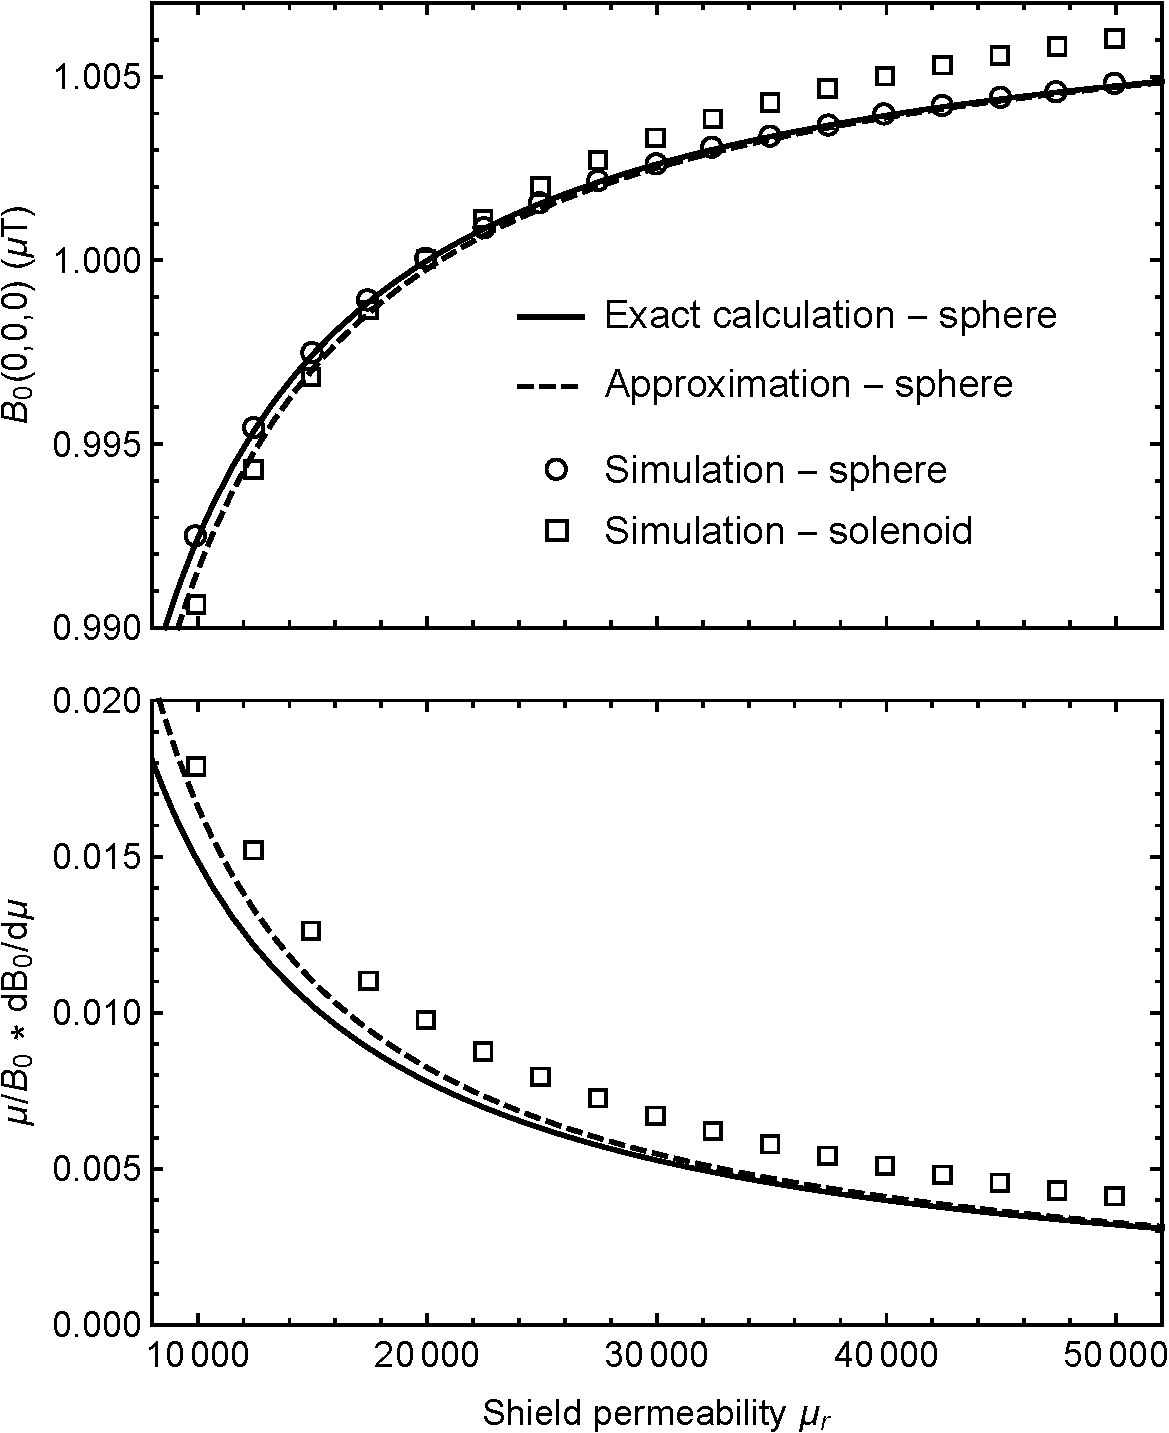
\includegraphics[width=0.7\textwidth]{Fig_combined-crop.pdf}
    \caption{Upper: Magnetic field at the coil center as a function of
      magnetic permeability of the surrounding magnetic shield for a
      geometry similar to the ILL nEDM experiment as discussed in the
      text.  Lower: $\frac{\mu}{B_0}\frac{dB_0}{d\mu}$
      vs.~permeability.  The solid curve is the exact calculation for
      the ideal spherical coil and shield from
      Ref.~\cite{bidinosti2014passive}; the dashed curve is the
      approximation of Eq.~\ref{Csphere}. The circles and squares are
      the FEMM-based simulations for the spherical and solenoidal
      geometries with discrete currents.  Since the spherical
      simulation was in agreement with the calculation, it is omitted
      from the lower graph.  For the exact calculation and the two
      simulations, currents were chosen to give $B_0=1~\mu$T at
      $\mu_r=20,000$.}
    \label{fig:Magnetic_Field}
    \end{center}
\end{figure} 


In the first simulation, the same spherical geometry was used as for
the analytic calculations.  However, the surface current was
discretized to 50 individual current loops, inscribed onto a sphere,
and equally spaced vertically (i.e.~a discrete sine-theta coil). A
square wire profile of side length 1~mm was used. As shown in
Fig.~\ref{fig:Magnetic_Field}, this simulation gave excellent
agreement with the analytic calculations.  In the second simulation, a
solenoid coil and cylindrical shield (length/radius~=~2) were used
with the same dimensions as above.  Similarly, the coil was modelled
as 50 evenly spaced current loops, with the distance from an end loop
to the inner face of the shield endcap being half the inter-loop
spacing.  In the limit of tight-packing (i.e., a continuous surface
current) and infinite $\mu$, the image currents in the end caps of the
shield act as an infinite series of current loops, giving the ideal
uniform field of an infinitely long
solenoid~\cite{lambert1975magnetically,sumner1987calculation}. As shown in
Fig.~\ref{fig:Magnetic_Field}, the result is similar to the spherical
case, with differences of order one part per thousand and a somewhat
steeper slope of $B_0(\mu_r)$.

Fig.~\ref{fig:Magnetic_Field} (lower) shows the normalized slope
$\frac{\mu}{B_0}\frac{dB_0}{d\mu}$ of the curves from
Fig.~\ref{fig:Magnetic_Field} (upper).  In ancillary measurements of
shielding factors (discussed briefly in
Section~\ref{sec:previousmeasurement}), we found $\mu_r=20,000$ to
offer a reasonable description of the quasistatic shielding factor of
our shield.  Using this value as the magnetic permeability of our
shield material, Fig.~\ref{fig:Magnetic_Field} (lower) shows that
$\frac{\mu}{B_0}\frac{dB_0}{d\mu}$ varies by about 20\% (from 0.008 to
0.01) for the spherical vs.~solenoidal geometries.  We adopt the value
$\frac{\mu}{B_0}\frac{dB_0}{d\mu}=0.01$ as an estimate of this slope
in our discussions in Section~\ref{sec:relationship}, acknowledging
that the value depends on the coil and shield design.

For a high-$\mu$ innermost shield, the magnetic field lines emanating
from the coil all return through the shield.  This principle can be
used to estimate the magnetic field $B_m$ inside the shield material,
and in our studies gave good agreement with FEA-based simulations.
For the solenoidal geometry previously described and used for the
calculations in Fig.~\ref{fig:Magnetic_Field}, $B_m$ is largest in the
side walls of the solenoidal flux return, attaining a maximum value of
170~$\mu$T.  If we assume $\mu_r$=20,000, the $H_m$ field is
0.007~A/m.  Typically the shield is degaussed (idealized) with the
internal coil energized. After degaussing, $B_m$ must be approximately
the same, since essentially all flux returns through the shield.
However, the $H_m$ field may become significantly smaller because
after degaussing, it must fall on the ideal magnetization curve in
$B_m-H_m$ space.  (For a discussion of the ideal magnetization curve,
refer to Ref.~\cite{bozorth1993ferromagnetism} and see
Fig.~\ref{fig:bh}.)  In principle, the $H_m$ field could be reduced by
an order of magnitude or more, depending on the steepness of the ideal
magnetization curve near the origin.  Thus $B_m=170~\mu$T and
$H_m<0.007$~A/m set a scale for the relevant values for nEDM
experiments.  Furthermore, the field in the nEDM measurement volume,
as well as in the magnetic shield, must be stable for periods of
typically hundreds of seconds (corresponding to frequencies
$<0.01$~Hz). This sets the relevant timescale for magnetic properties
most relevant to nEDM experiments.


\begin{figure}[h!]
  \centering
  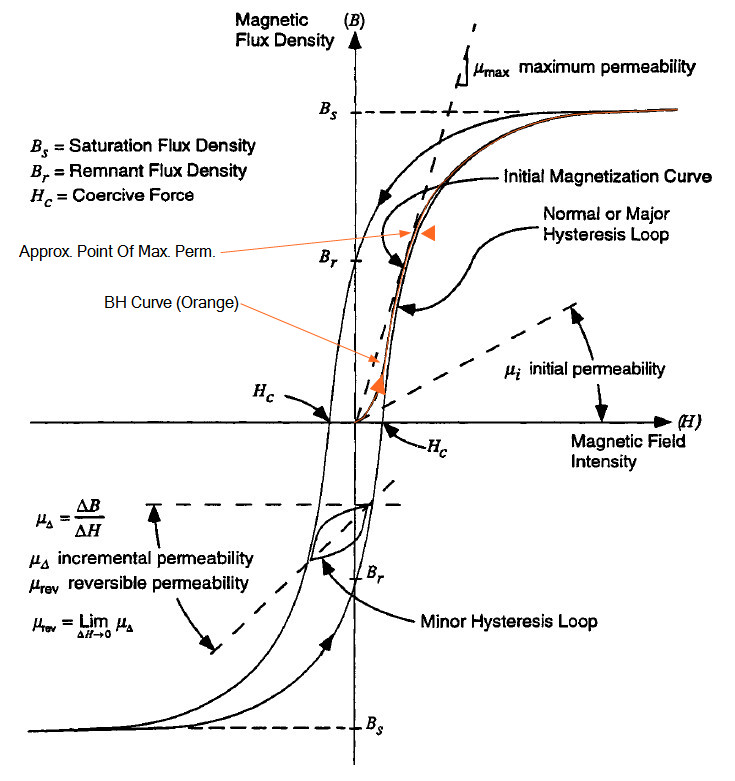
\includegraphics[width=0.8\textwidth]{bh.jpg}
  \caption{The hysteresis or $B-H$ curve. Some commonly used
    terminology is shown. $H_c$ or coercivity is a measure of the
    ability of the material to withstand external magnetic fields and
    is at $B=0$. Initial permeability or $\mu_i$ is the slope of the
    initial magnetization curve. The initial magnetization or
    idealization curve is achievable after degaussing the high $\mu$
    material. }
  \label{fig:bh}
\end{figure}
